% Few-Shot Progression Plot für LaTeX-Thesis
% Automatisch generiert - NICHT MANUELL BEARBEITEN

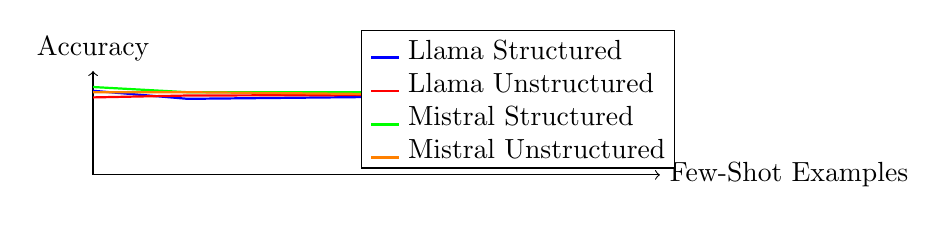
\begin{tikzpicture}[scale=1.2]
% Koordinaten
\coordinate (llamastructuredzero) at (0,0.890);
\coordinate (llamastructuredone) at (1,0.805);
\coordinate (llamastructuredthree) at (3,0.825);
\coordinate (llamastructuredfive) at (5,0.805);
\coordinate (llamaunstructuredzero) at (0,0.820);
\coordinate (llamaunstructuredone) at (1,0.840);
\coordinate (llamaunstructuredthree) at (3,0.845);
\coordinate (llamaunstructuredfive) at (5,0.840);
\coordinate (mistralstructuredzero) at (0,0.930);
\coordinate (mistralstructuredone) at (1,0.875);
\coordinate (mistralstructuredthree) at (3,0.875);
\coordinate (mistralstructuredfive) at (5,0.895);
\coordinate (mistralunstructuredzero) at (0,0.875);
\coordinate (mistralunstructuredone) at (1,0.875);
\coordinate (mistralunstructuredthree) at (3,0.855);
\coordinate (mistralunstructuredfive) at (5,0.745);

% Achsen
\draw[->] (0,0) -- (6,0) node[right] {Few-Shot Examples};
\draw[->] (0,0) -- (0,1.1) node[above] {Accuracy};

% Plots
\draw[thick,blue] plot coordinates {(llamastructuredzero) (llamastructuredone) (llamastructuredthree) (llamastructuredfive)};
\draw[thick,red] plot coordinates {(llamaunstructuredzero) (llamaunstructuredone) (llamaunstructuredthree) (llamaunstructuredfive)};
\draw[thick,green] plot coordinates {(mistralstructuredzero) (mistralstructuredone) (mistralstructuredthree) (mistralstructuredfive)};
\draw[thick,orange] plot coordinates {(mistralunstructuredzero) (mistralunstructuredone) (mistralunstructuredthree) (mistralunstructuredfive)};

% Legende
\node[draw,fill=white,align=left] at (4.5,0.8) {
\textcolor{blue}{\rule{1em}{1pt}} Llama Structured\\
\textcolor{red}{\rule{1em}{1pt}} Llama Unstructured\\
\textcolor{green}{\rule{1em}{1pt}} Mistral Structured\\
\textcolor{orange}{\rule{1em}{1pt}} Mistral Unstructured
};
\end{tikzpicture}
